\documentclass{beamer}
%Для защит онлайн лучше использовать разрешение 16x9
%\documentclass[aspectratio=169]{beamer}

\input{preamble.tex}

% То, что в квадратных скобках, отображается внизу по центру каждого слайда. 
\title[Разработка приложения]{Разработка мобильного приложения для развития музыкальных навыков}

% То, что в квадратных скобках, отображается в левом нижнем углу. 
\institute[СПбГУ]{}

% То, что в квадратных скобках, отображается в левом нижнем углу.
\author[Зайцев Дмитрий]{Зайцев Дмитрий Сергеевич, группа 22.Б11-мм}
 
\begin{document}
{
\setbeamertemplate{footline}{}
% Лого университета или организации, отображается в шапке титульного листа
\begin{frame}
  \includegraphics[width=1.4cm]{pictures/SPbGU_Logo.png}
\vspace{-35pt}
\hspace{-10pt}
\begin{center}
   \begin{tabular}{c}
        \scriptsize{Санкт-Петербургский государственный университет} \\
        \scriptsize{Кафедра системного программирования}
    \end{tabular}
\titlepage
\end{center}

\btVFill

{\scriptsize
  % У научного руководителя должна быть указана научная степень
   \textbf{Научный руководитель:} старший преподаватель СПБГУ Сартасов С. Ю. \\
 }
\begin{center}
  \vspace{5pt}
  \scriptsize{Санкт-Петербург\\
                 2023}
  \end{center}

\end{frame}
}

\begin{frame}[fragile]  
  \frametitle{Введение}
  \begin{itemize}
    \item Интерес к музыке никогда не падает, сейчас это одно из самых популярных хобби
    \item Изучение музыки -- трудоёмкий процесс, требующий наличия рядом опытного преподавателя
    \item Существует мало современных, эффективных решений для развития этих навыков
  \end{itemize}
\end{frame}
           
% Обязательный слайд: четкая формулировка цели данной работы и постановка задачи
% Описание выносимых на защиту результатов, процесса или особенностей их достижения и т.д.
\begin{frame}
  \frametitle{Постановка задачи}
  \textbf{Целью} работы является создание мобильного приложения, которое смогло бы облегчить
процесс формирования способности определения интервалов на слух.

  \textbf{Задачи}:
  \begin{enumerate}
    \item Обзор существующих решений
    \item Разработка архитектуры
    \item Создание приложения с первым обучающим режимом
  \end{enumerate}
\end{frame}                      
            
\begin{frame}  
  \frametitle{Существующие решения}
  \begin{itemize}
    \item В ходе работы был проведён анализ отзывов пользователей на несколько приложений с наибольшим числом скачиваний
    \item Рассмотрены приложения: Perfect ear, Functional Ear Trainer, My Ear Trainer 
  \end{itemize}
  
    \begin{itemize}
    \item Выводы
    \begin{itemize}
      \item Существует реальная потребность в приложениях, помогающих в освоении музыкальных навыков
      \item Ни одно из решений полностью не решает проблемы, для учащихся российских музыкальных школ ситуация ещё хуже
      \item При разработке приложений было принято также и множество хороших решений (гибкая настройка упражнений, наличие теоретического материала рядом с заданиями)
    \end{itemize}
  \end{itemize}  
    
\end{frame}
            
\begin{frame}  
  \frametitle{Используемые технологии}
  \begin{itemize}
    \item JVM
    \item Kotlin
    \item Android Studio
    \item Gradle
    \item JUnit 5
    \item Jetpack Compose
  \end{itemize}   
\end{frame}             
            
%Идеально, если есть по одному слайду на каждую поставленную задачу            

\begin{frame}
  \frametitle{Архитектура приложения}
  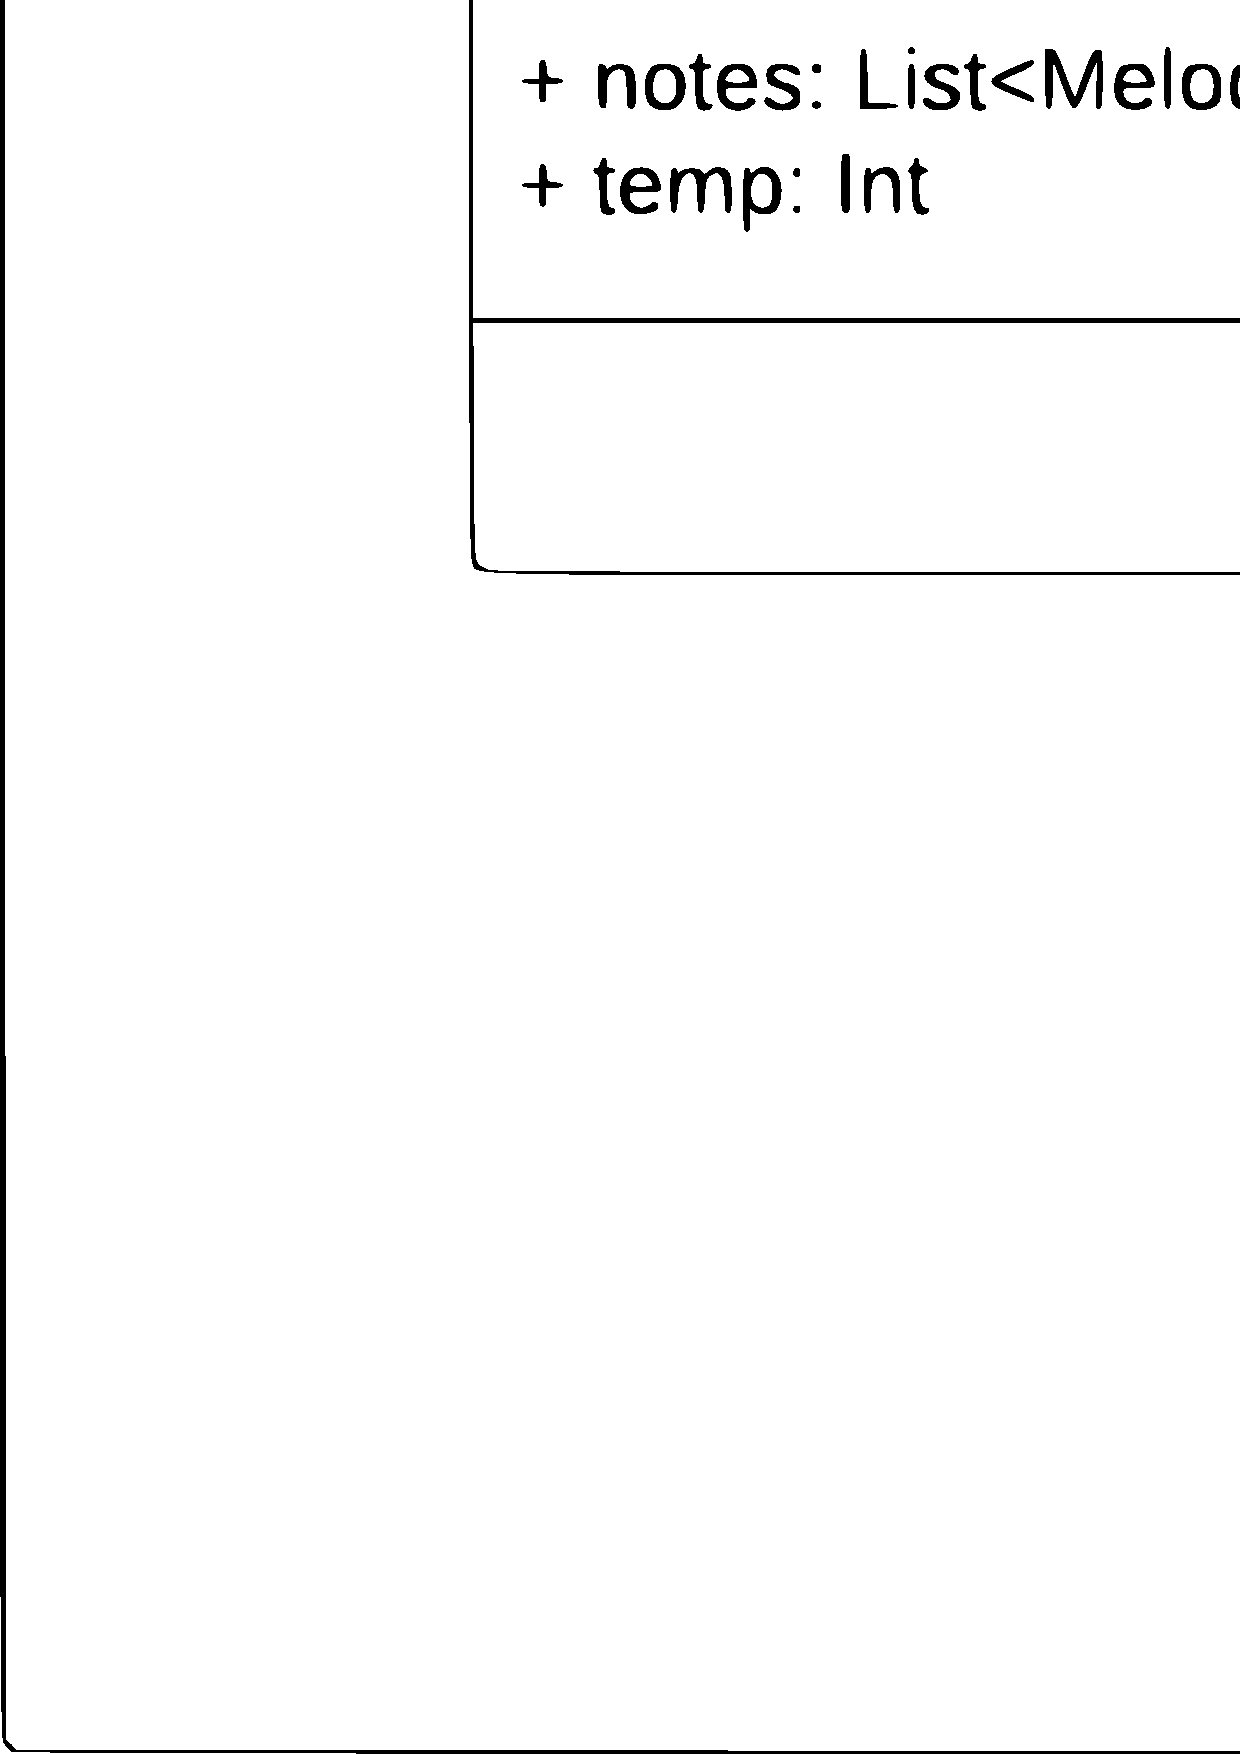
\includegraphics[width=\textwidth]{../images/UML.pdf}
\end{frame}

\begin{frame}
  \frametitle{Пользовательский интерфейс}
  \begin{tabular}{p{6cm} p{7cm}}
  Внешний вид упражнения & \hspace{13pt}Piano Checkbox \\
  \hspace{10pt}
  \includegraphics[width=0.3\textwidth]{../images/example3-eps-converted-to.pdf}&
  \vspace{-200pt}
  \includegraphics[width=0.3\textwidth]{../images/example1-eps-converted-to.pdf}\\
  &
  \vspace{-105pt}
  \hspace{15pt}Piano Keyboard\\&
  \vspace{-105pt}
  \includegraphics[width=0.3\textwidth]{../images/example4-eps-converted-to.pdf}
 \end{tabular}
\end{frame}

\begin{frame}
  \frametitle{Результаты}
  Были решены следующие задачи:
  \begin{itemize}
    \item Выполнен обзор существующих решений
    \item Разработана архитектура приложения
    \item Реализован первый обучающий режим
  \end{itemize}
\vspace{30pt}
Весь код есть в репозитории проекта (+ CI со сборкой APK): \url{https://github.com/d-zaytsev/android-app}
\end{frame}

\end{document}